\section{Введение в виртуализацию}

В данном руководстве описывается установка и настройка системы виртуализации OpenVZ\footnote{OpenVZ распространяется под лицензией GNU GPL v2.0} 
на базе Linux-дистрибутива CentOS 6.

На момент последней правки руководства, последняя версия CentOS, поддерживающая OpenVZ "--- 6.6.

Для полного понимания информации руководства, необходимо иметь базовые знания о виртуализации, а также иметь навыки работы в командной строке GNU/Linux.

Виртуализация "--- предоставление наборов вычислительных ресурсов или их логического объединения, абстрагированное от аппаратной реализации, и обеспечивающее изоляцию вычислительных процессов. 

Виртуализацию можно использовать в \cite{sevconf2014}:
\begin{itemize}
    \item Консолидации серверов (позволяет мигрировать с физических серверов на виртуальные, тем самым увеличивается коэффициент использования аппаратуры, что позволяет существенно сэкономить на аппаратуре, электроэнергии и обслуживании);
    \item Разработке и тестировании приложений (возможность одновременно запускать несколько различных ОС, это удобно при разработке кроссплатформенного ПО, тем самым значительно повышается качество, скорость разработки и тестирования приложений);
    \item Бизнесе (использование виртуализации в бизнесе растет с каждым днем и постоянно находятся новые способы применения этой технологии, например, возможность безболезненно сделать снапшот\footnote{Снапшот (англ. snapshot) "--- снимок состояния виртуальной машины (ВМ) в определенный момент времени. Сюда входят настройки ВМ, содержимое памяти и дисков} и быстро восстановить систему в случае сбоя);
    \item Организации виртуальных рабочих станций (так называемых <<тонких клиентов>>\footnote{Тонкий клиент (англ. thin client) "--- бездисковый компьютер-клиент в сетях с клиент-серверной или терминальной архитектурой, который переносит все или большую часть задач по обработке информации на сервер}).
\end{itemize}

Общая схема взаимодействия виртуализации с аппаратурой и программным обеспечением (ПО) представлена на рис.~\ref{pic:virt_scheme}.
\begin{figure}[ht]
    \centering
	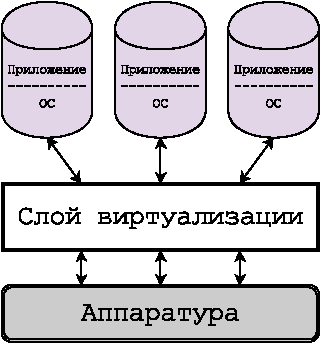
\includegraphics[width=0.4\linewidth]{virt_scheme.pdf}
	\caption{Схема взаимодействия виртуализации с аппаратурой и ПО}\label{pic:virt_scheme}
\end{figure}

Взаимодействие приложений и операционной системы (ОС) с аппаратным обеспечением осуществляется через абстрагированный слой виртуализации. 

Существует несколько подходов организации виртуализации:
\begin{itemize}
    \item Эмуляция оборудования (QEMU, Bochs, Dynamips);
    \item Полная виртуализация (KVM, HyperV, VirtualBox);
    \item Паравиртуализация (Xen, L4, Trango);
    \item Виртуализация уровня ОС (LXC, OpenVZ, Jails, Solaris Zones).
\end{itemize}

\textbf{Эмуляция оборудования} является самым сложным и трудоемким методом виртуализации (рис.~\ref{pic:emulation}).
Однако, большим преимуществом для данного метода является, к примеру, управление неизмененной ОС, предназначенной для PowerPC на системе с ARM процессором.
\begin{figure}[ht]
    \centering
	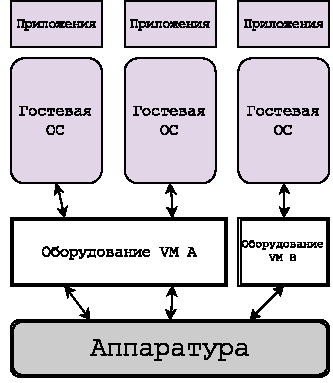
\includegraphics[width=0.4\linewidth]{emulation.pdf}
	\caption{Эмуляция оборудования моделирует аппаратные средства}\label{pic:emulation}
\end{figure}

В \textbf{полной виртуализации}, поверх уже установленной ОС, устанавливается программа-гипервизор\footnote{Гипервизор (англ. hypervisor)"--- программа или аппаратная схема, позволяющая одновременное, параллельное выполнение нескольких ОС на одном и том же компьютере, обеспечивает изоляцию операционных систем друг от друга}, которая осуществляет взаимосвязь между гостевыми ОС и хост-компьютером (рис.~\ref{pic:full_virt}).
\begin{figure}[ht]
    \centering
	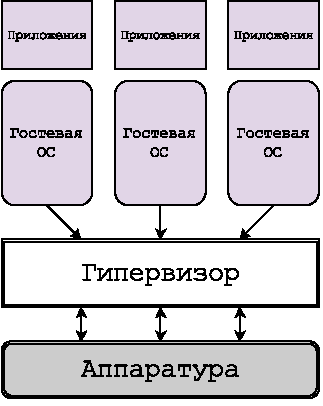
\includegraphics[width=0.4\linewidth]{full_virt.pdf}
	\caption{Полная виртуализация использует гипервизор}\label{pic:full_virt}
\end{figure}

Преимуществом технологии полной виртуализации является установка различных ОС, а недостатком "--- меньшая производительность, за счет накладных расходов на гипервизор, а также понижение скорости работы с подсистемой ввода/вывода из-за необходимости изоляции.

\textbf{Паравиртуализация} имеет некоторые сходства с полной виртуализацией. 
В данном методе также используется гипервизор для разделения доступа к аппаратуре, но объединяется код, касающийся виртуализации, в ОС \cite{virtuallinux} (рис.~\ref{pic:paravirt}).
\begin{figure}[ht]
    \centering
	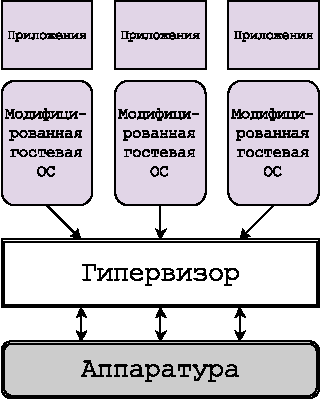
\includegraphics[width=0.4\linewidth]{paravirt.pdf}
	\caption{Паравиртуализация разделяет процесс с гостевой ОС}\label{pic:paravirt}
\end{figure}

Недостатком паравиртуализации является необходимость изменения гостевой ОС для гипервизора, однако таким образом гораздо увеличивается производительность.

\textbf{Виртуализация уровня операционной системы}  не нуждается в гипервизоре. 
Для ее работы необходимо модифицированное ядро на хост-системе с набором патчей и утилит для управления контейнерами\footnote{Контейнер или VPS/VDS (англ. Virtual Private/Dedicated Server) "--- виртуальный выделенный сервер, эмулирует работу физического сервера} (рис.~\ref{pic:cont_virt}).
\begin{figure}[ht]
    \centering
	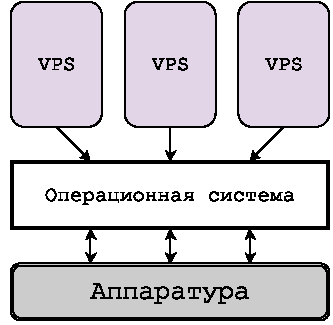
\includegraphics[width=0.4\linewidth]{cont_virt.pdf}
	\caption{Виртуализация уровня ОС изолирует серверы}\label{pic:cont_virt}
\end{figure}

За счет того, что контейнер напрямую взаимодействует с ядром, а не через гипервизор, обеспечивается максимальное быстродействие. Но, так как для всех контейнеров используется общее ядро, то нет возможности использовать разные ОС в контейнерах.

OpenVZ "--- технология виртуализации на уровне ОС. 
Позволяет создавать множество защищенных, изолированных друг от друга виртуальных сред (VE) на одном узле. 

Каждый контейнер ведет себя так же, как автономный сервер и имеет собственные файлы, процессы, сеть (IP адреса, правила маршрутизации и~т.~д.).
В отличие от KVM или Xen, OpenVZ использует одно ядро, которое является общим для всех виртуальных сред.

Контейнеры можно разделить на две составляющие:
\begin{itemize}
    \item Ядро (namespaces, cgroups);
    \item Пользовательские утилиты (vzctl, vzquota, vzdump, ...).
\end{itemize}
 
\textbf{namespaces} "--- пространства полностью изолированных имен, позволяющие безопасно изолировать дисковое пространство, процессы, пользователей, имя компьютера (hostname) и~т.~д.

\textbf{cgroups} "--- механизм контроля за ресурсами, позволяющий управлять памятью и распределять процессорное время.

Для удобства управления контейнерами можно использовать консольные утилиты (vzctl), либо управлять ими через Web-браузер (OpenVZ Web Panel, ISP VEmanager).

Проведенные тестирования показывают, что OpenVZ является одним из наиболее актуальных решений на рынке виртуализации, так как показывает внушительные результаты в различных тестированиях \cite{padala2007performance}.
Один из таких тестов \cite{openvzperformance} приведен на рис.~\ref{pic:openvz_tests}.

\begin{figure}[ht]
    \centering
	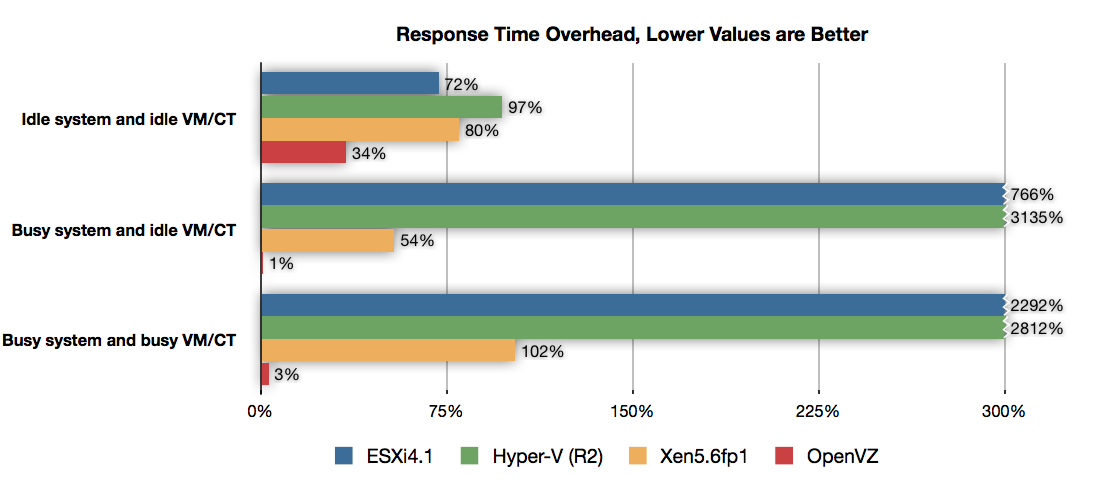
\includegraphics[width=\linewidth]{Response_time_v2.png}
	\caption{Время отклика системы (меньше "--- лучше)}\label{pic:openvz_tests}
\end{figure}

На графике можно наблюдать, что проводилось три теста с нагрузкой на систему и виртуальную машину (ВМ), без нагрузки на систему и ВМ, с нагрузкой на ВМ и без нагрузки на систему.
Во всех трех тестах OpenVZ показал результаты наименьшего времени отклика. 
В этих тестах ESXi и Hyper-V показывают оверхед\footnote{Оверхед (англ. overhead) "--- неизбежные накладные расходы памяти или процессорного времени} 700---3000\%, когда у OpenVZ всего 1---3\%.

\clearpage
